\documentclass[%
a4paper,							% alle weiteren Papierformat einstellbar
%landscape,						% Querformat
12pt,								% Schriftgröße (12pt, 11pt (Standard))
%BCOR1cm,							% Bindekorrektur, bspw. 1 cm
%DIVcalc,							% führt die Satzspiegelberechnung neu aus
%											  s. scrguide 2.4
%twoside,							% Doppelseiten
%twocolumn,						% zweispaltiger Satz
%halfparskip*,				% Absatzformatierung s. scrguide 3.1
parskip=half,
%headsepline,					% Trennline zum Seitenkopf	
%footsepline,					% Trennline zum Seitenfuß
%titlepage,						% Titelei auf eigener Seite
%normalheadings,			% Überschriften etwas kleiner (smallheadings)
%idxtotoc,						% Index im Inhaltsverzeichnis
%liststotoc,					% Abb.- und Tab.verzeichnis im Inhalt
%bibtotoc,						% Literaturverzeichnis im Inhalt
%abstracton,					% Überschrift über der Zusammenfassung an	
%leqno,   						% Nummerierung von Gleichungen links
%fleqn,								% Ausgabe von Gleichungen linksbündig
%draft								% überlangen Zeilen in Ausgabe gekennzeichnet
]
{article}


%% Deutsche Anpassungen %%%%%%%%%%%%%%%%%%%%%%%%%%%%%%%%%%%%%
\usepackage[ngerman]{babel}
\usepackage[T1]{fontenc}
\usepackage[utf8]{inputenc}
\usepackage{lmodern} %Type1-Schriftart für nicht-englische Texte
\usepackage{textcomp}

%% Konstanten %%%%%%%%%%%%%%%%%%%%%%%%%%%%%%%%%%%%%
\newcommand{\course}{Labor Projekt}
\newcommand{\exercise}{RISC-V RV32I Mikrocontroller}
\newcommand{\topic}{Dokumentation}
\newcommand{\authorname}{Guillaume Fournier-Mayer}
\newcommand{\matnum}{Tinf-101922}
\newcommand{\fachsemester}{Fachsemester 7}
\newcommand{\verwaltungssemester}{Verwaltungssemester 11}


%% Packages für Grafiken & Abbildungen %%%%%%%%%%%%%%%%%%%%%%
\usepackage{graphicx}
\usepackage{eso-pic}
\usepackage{float}


%% Hyperref %%%%%%%%%%%%%%%%%%%%%%%%%%%%%%%%%%%%%%%%%%%%%%%%%
\usepackage[final, backref=false, pagebackref=false, bookmarks=true]{hyperref}

\hypersetup{ %Ä=\304; Ö=\326; Ü=\334; ä=\344; ö=\366; ü=\374; ß=\377
  pdfauthor={\authorname},
  pdftitle={\course{}: \exercise{} \topic{}},
  pdfsubject={\course{}: \exercise{} \topic{}},
  pdfproducer={MiKTeX},
  pdfview=FitV,             % Fit, FitH, FitV
  pdfstartview=FitV,        % PDF-Viewer benutzt beim Start bestimmte Seitenbreite
                            % (Fit, FitH, FitV)
  pdfpagemode=UseOutlines,  % PDF-Viewer startet ohne Inhaltsverzeichnis et.al.
                            % (FullScreen, UseOutlines, None)
  linkcolor=black,          % Für Links in der gleichen Seite
  urlcolor=blue,            % Für Links auf URL’s
  breaklinks=false,         % Links dürfen umgebrochen werden
  colorlinks=true,
  citecolor=black,          % Farbe für \cite
  citebordercolor=0 0 0,
  filebordercolor=0 0 0,
  linkbordercolor=0 0 0,
  menubordercolor=0 0 0,
  urlbordercolor=0 0 0,
  pdfhighlight=/I,
  pdfborder=0 0 0,          % keine Box um die Links!
  bookmarksnumbered=false,
  bookmarksopen=true
}

%% Geometry %%%%%%%%%%%%%%%%%%%%%%%%%%%%%%%%%%%%%%%%%%%%%%%%%
\usepackage[a4paper]{geometry}
\geometry{includeheadfoot, headheight = 17mm, textwidth = 16cm, textheight = 23cm}

%% Subfigure %%%%%%%%%%%%%%%%%%%%%%%%%%%%%%%%%%%%%%%%%%%%%%%%%
\usepackage{subfigure}

%% Listigs %%%%%%%%%%%%%%%%%%%%%%%%%%%%%%%%%%%%%%%%%%%%%%%%%%
\usepackage{listings}
\lstset{
	language=C,
  basicstyle=\ttfamily,
  commentstyle=\ttfamily,
  backgroundcolor=\color[gray]{0.9},
  numbers=left,
  stepnumber=1,
  showstringspaces=false,
  breaklines=true,
  columns=fullflexible,
  frame=single,
}
%% TABLE %%%%%%%%%%%%%%%%%%%%%%%%%%%%%%%%%%%%%%%%%%%%%%%%%%%
\usepackage{longtable}

%% Header %%%%%%%%%%%%%%%%%%%%%%%%%%%%%%%%%%%%%%%%%%%%%%%%%%%
\usepackage{fancyhdr}
\pagestyle{fancy}
\renewcommand{\headrulewidth}{0.3pt}
\renewcommand{\footrulewidth}{0.3pt}
% Beschriftung der Kopf- und Fußzeilen (alle Seiten gleich)
\fancyhead[L]{\course{}: \exercise{}}
\fancyhead[C]{}
\fancyhead[R]{
\includegraphics[height=1.5cm]{img/fhlogo.pdf}}
\fancyfoot[L]{\authorname{} - \matnum}
\fancyfoot[C]{}
\fancyfoot[R]{\thepage}


%% Zitate %%%%%%%%%%%%%%%%%%%%%%%%%%%%%%%%%%%%%%%%%%%%%%%%%%%%%

\usepackage[backend=biber,style=alphabetic,]{biblatex}
\addbibresource{literatur.bib}

\begin{document}
\AddToShipoutPicture{
\includegraphics{img/Deckblatt.pdf}}
\begin{titlepage}

  \centering 
  { \Huge $ $ \\ }
  \vspace{5cm}
	{ \Huge
  	\course{}\\
  	\vspace{1cm}
  	\LARGE
    \exercise{}\\
    \topic{}\\}
  \vspace{8cm}
  \authorname\\
  \vspace{1cm}
  Wedel, den \today{}

\end{titlepage}
\ClearShipoutPicture
\tableofcontents
\newpage
\setcounter{page}{1}
\part{Benutzerhandbuch}
    \section{Ablaufbedingungen}
    Um den Mikrocontroller in Betrieb zu nehmen wird folgeden Soft- und Hardware benötigt.
   

    \subsection{Software}
        Als Betriebsystem wird ein Linux Betriebsystem benötigt.
        \begin{center}
            \begin{longtable}{| l | l | l |}
                \hline
                    Software & Version & Quelle \\
                \hline
                    Quartus Prime Lite & 20.1.1 & \href{https://fpgasoftware.intel.com/?edition=lite}{Intel}\\
                \hline
                    Arrow USB Programmer & 2.4.1-1 & \href{https://wiki.trenz-electronic.de/display/PD/Arrow+USB+Programmer#ArrowUSBProgrammer-DownloadSetupFiles}{Trenz Electronics}\\
                \hline
                    RISC-V GCC Toolchain & 9.2.0 & \href{https://github.com/riscv/riscv-gnu-toolchain}{RISC-V Organisation}\\
                \hline
                \caption{Benötigte Software für Inbetriebnahme}
            \end{longtable}
        \end{center}

    \subsection{Hardware}
        \begin{center}
            \begin{longtable}{| l | l | l |}
                \hline
                    Hardware & Version & Quelle \\
                \hline
                    TEI0003 - CYC1000 & 0.2 & \href{https://wiki.trenz-electronic.de/display/PD/TEI0003+Getting+Started}{Trenz Electorincs}\\
                \hline
                    Micro-USB-Kabel & 2.0 & \\
                \hline
                \caption{Benötigte Hardware für Inbetriebnahme}
            \end{longtable}
        \end{center}
    \chapter{Bedienungsanleitung}

    \section{Öffnen des Projektes}
        Zunächst wird \textit{Quartus Prime Lite} gestartet.
        Sobald das Hauptfenster geöffnet wurde kann über den Menüpunkt \textit{File}
        der Untermenüpunkt \textit{Open Project}, wie in Abbildung \ref{fig:quartus_open_project} gezeigt,
        geklickt werden. Daraufhin öffnet sich ein Dateibrowser (Abbildung \ref{fig:quartus_select_project})
        durch den das Projekt ausgewählt werden kann.
        Der relative Pfad des Projektes im Repository ist dabei \textit{RiscV-i32/CPU/Design/RiscV.qpf}
        
        \begin{figure}[H]
            \centering
            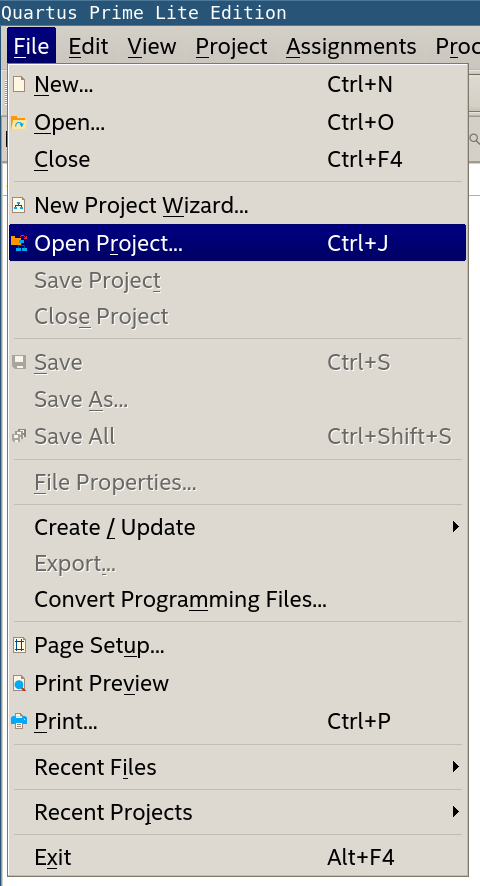
\includegraphics[scale=0.6]{img/quartus_open_project.png}
            \caption{Öffnen des Projektes in Quartus}
            \label{fig:quartus_open_project}
        \end{figure}

        \begin{figure}[H]
            \centering
            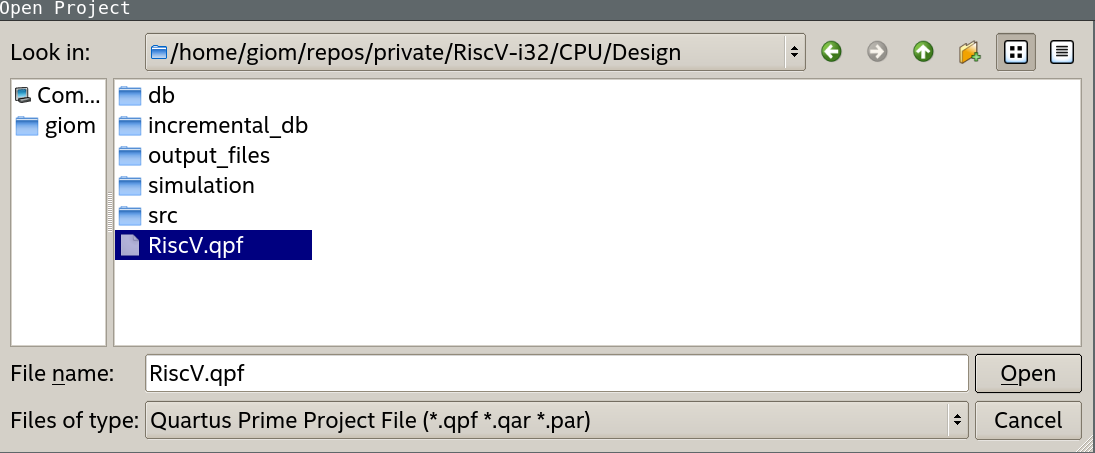
\includegraphics[scale=0.6]{img/quartus_select_project.png}
            \caption{Öffnen des Projektes in Quartus}
            \label{fig:quartus_select_project}
        \end{figure}


    \section{Bauen des Projektes}
        Sobald sich das Projekt erfolgreich geöffnet hat, kann das Bauen über einen Klick
        auf das \textit{Play}-Symbol (Abbildung \ref{fig:quartus_play}) gestartet werden. Das eigentliche Bauen kann, je nach
        Leistung des Rechners mehrere Minuten dauern. Dabei wird der Status im unteren
        Fensterdrittel angezeigt. War das Bauen erfolgreich wird die Meldung
        \textit{Quartus Prime Full Compilation was successful} (Abbildung \ref{fig:quartus_build_sucessful})
        angezeigt.

        \begin{figure}[H]
            \centering
            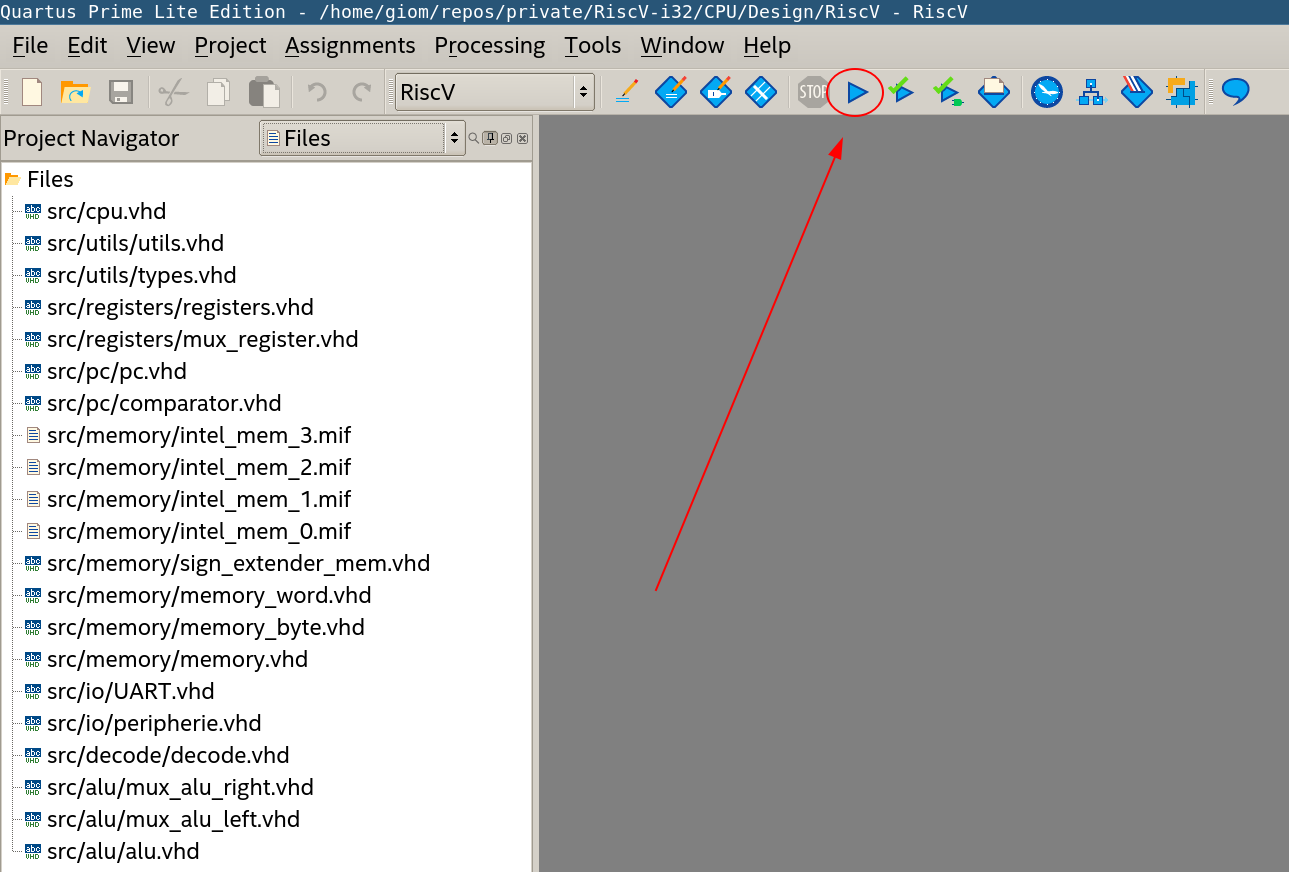
\includegraphics[scale=0.6]{img/quartus_build.png}
            \caption{Bauen des Projektes in Quartus}
            \label{fig:quartus_play}
        \end{figure}

        \begin{figure}[H]
            \centering
            
\includegraphics[scale=0.6]{img/quartus_build_sucessfull.png}
            \caption{Erfolgreiches Bauen des Projektes in Quartus}
            \label{fig:quartus_build_sucessful}
        \end{figure}


    \section{Flashen des FPGAs}

    Zunächst muss das FPGA-Board über USB angeschlossen werden. Zusätzlich muss der Treiber schon installiert sein.
    Ist dies der Fall kann über den Menüpunkt \textit{Tools} der Untermenüpunkt \textit{Programmer}
    ausgewählt werden. (Abbildung \ref{fig:quartus_programmer})
    Dadurch öffnet sich der Programmer (Abbildung \ref{fig:quartus_programmer_window})
    und die Hardware kann durch einen Klick auf \textit{Hardware Setup} eingerichtet werden.
    Ein weiteres Fenster öffnet sich (Abbildung \ref{fig:quartus_programmer_select_hardware}).
    Ein Doppelklick auf \textit{Arrow-USB-Blaster (1)} wählt das FPGA-Board als Ziel für den Programmer.
    Dies kann durch \textit{Currently selected Hardware (2)} bestätigt werden. Ein weiterer Klick 
    \textit{close} schließt das Fenster wieder. Nun kann über \textit{Start}
    (Abbildung \ref{fig:quartus_programmer_start}) das eigentliche Flashen beginnen.
    Eine visuelles Rückmeldung bietet hierbei der Ladebalken \textit{Progress}.
    

    \begin{figure}[H]
        \centering
        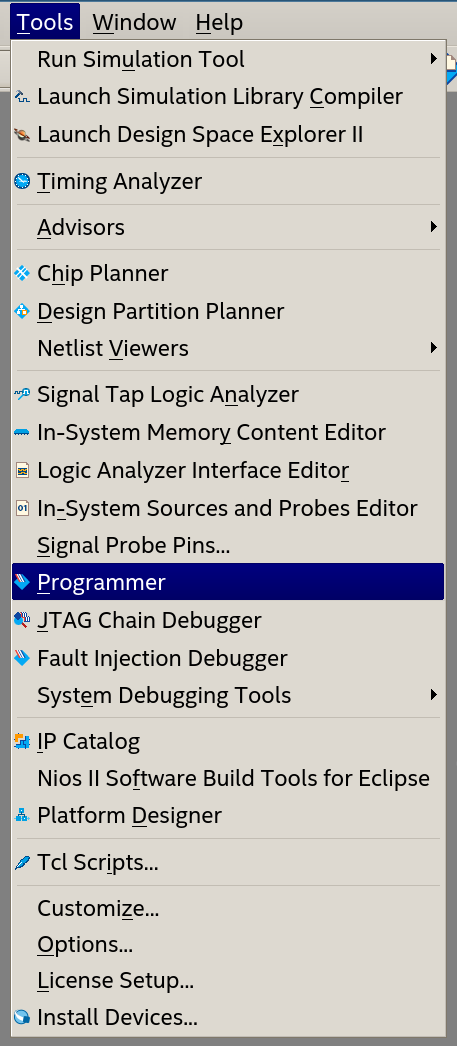
\includegraphics[scale=0.6]{img/quartus_programmer.png}
        \caption{Öffnen des Programmers in Quartus}
        \label{fig:quartus_programmer}
    \end{figure}

    \begin{figure}[H]
        \centering
        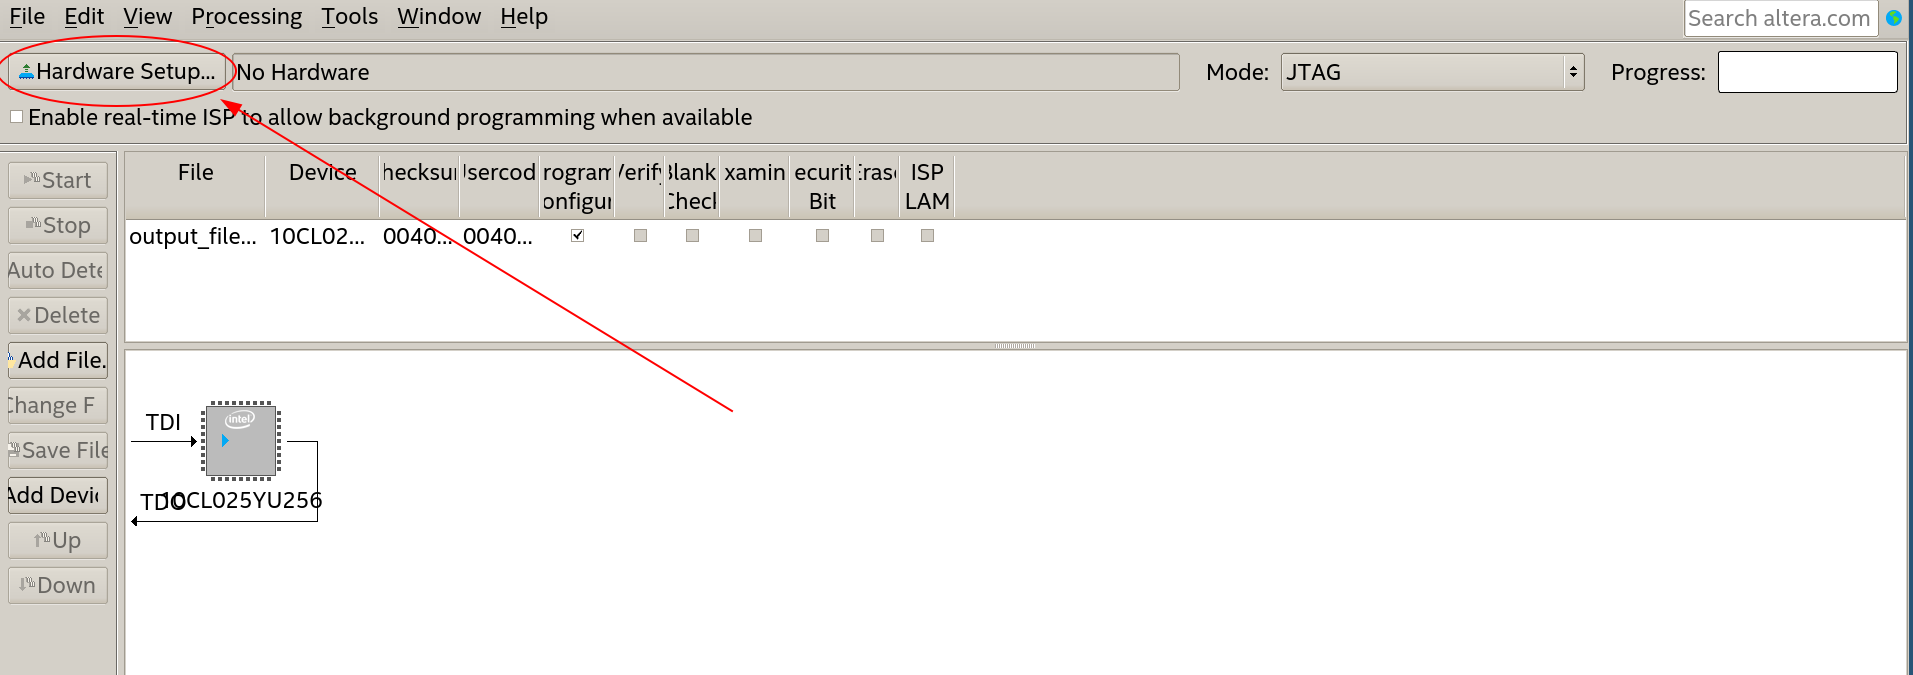
\includegraphics[scale=0.6]{img/quartus_programmer_select_hardware.png}
        \caption{Einrichten der Hardware in Quartus}
        \label{fig:quartus_programmer_window}
    \end{figure}

    \begin{figure}[H]
        \centering
        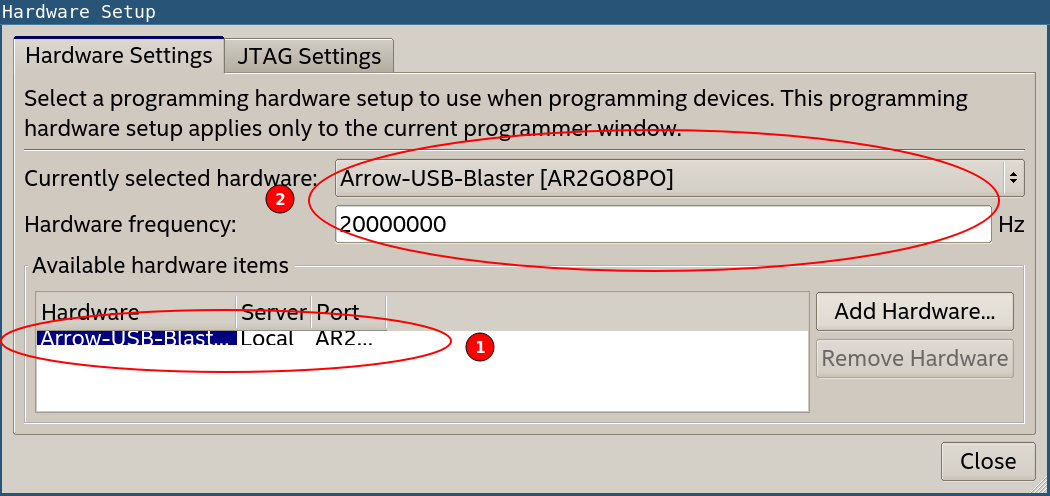
\includegraphics[scale=0.6]{img/quartus_programmer_select_hardware2.png}
        \caption{Einrichten der Hardware in Quartus}
        \label{fig:quartus_programmer_select_hardware}
    \end{figure}

    \begin{figure}[H]
        \centering
        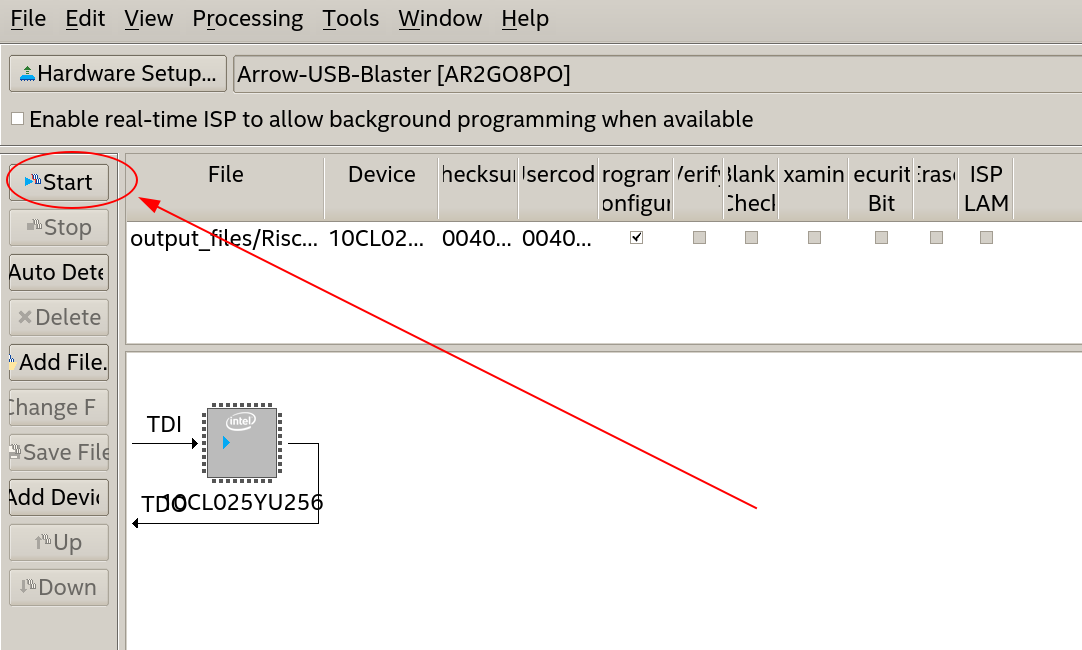
\includegraphics[scale=0.6]{img/quartus_programmer_start.png}
        \caption{Starten des Flashens des FPGAs}
        \label{fig:quartus_programmer_start}
    \end{figure}


    \section{Kompilieren des Programmcodes}
    \section{Flashen des Mikrocontrollers}




\part{Programmiererhandbuch}

\chapter{Motivation}

    \section{RISC-V}
        \textit{RISC-V} ist eine offene und erweiterbare Befehlssatzarchitektur (ISA) die sich an dem
        \textit{RISC (Reduced Instruction Set Computer)} Designprinzip orentiert.
        Dank der freizügigen \textit{BSD-Lizenz} ist es, im Gegensatz zu bspw. der \textit{x86} ISA von \textit{Intel},
        jedem erlaubt \textit{RISC-V} Mikroprozessoren zu entwerfen, herzustellen und zu verkaufen.
        Die Lizenz erlaubt es zusätzlich den Befehlssatz nach belieben zu erweitern und somit
        optimal an eine Hardwarearchitektur anzupassen.
        In Tabelle \ref{label:riscv-base} werden die Grundbefehlssätze von RISC-V dargestellt.
        Darüber hinaus besitzt RISC-V noch zusätzliche Befehlssätze die z.B. Hardwaremultiplikation
        oder Fließkomma-Arithmetik erlauben. \cite{riscv-isa-specs}
        
        \begin{center}
            \begin{longtable}{| l | l | l |}
                \hline
                    Name & Beschreibung & Version \\
                \hline
                    RV32I & 32Bit Integer Basisbefehlssatz mit 32 Registern & 2.1 (Ratifiziert)\\
                \hline
                    RV32E & 32Bit Integer Basisbefehlssatz mit 16 Registern (Eingebettete Systeme) & 1.9 (Offen)\\
                \hline
                    RV64I & 64Bit Integer Basisbefehlssatz & 2.1 (Ratifiziert)\\
                \hline
                    RV128I & 128Bit Integer Basisbefehlssatz & 1.7 (Offen)\\
                \hline
                \caption{RISC-V Grundbefehlssätze}
                \label{label:riscv-base}
            \end{longtable}
        \end{center}

    \section{FPGA (Field Programmable Gate Array)}
        Ein FPGA, (Field Programmable Gate Array) ist ein integrierter Schaltkreis (IC) der Digitaltechnik,
        in welchen eine logische Schaltung geladen werden kann.
        Im Vergleich zu der Programmierung von Computern oder Mikrocontrollern wird die Schaltungsstruktur eines FPGAs durch eine
        Hardwarebeschreibungssprache (z.B. VHDL) beschrieben. Man spricht daher auch von der Konfiguration des FPGA.
        Ohne diese hat der Baustein keine Funktion. \cite{fpga-wiki}
        \\
        Durch einen FPGA ist es somit möglich einen \textit{RISC-V} Befehlssatz in VHDL zu formulieren und auf Hardware zu testen,
        ohne Kosten für eine Fertigung des Chips aufzubringen.


\section{Aufgabenstellung}
    In dem Laborprojekt soll ein Mikrocontroller entwickelt werden der den \textit{RV32I} Befehlssatz implementiert.
    Dieser soll auf ein FPGA board hochgeladen werden können und Programmcode ausführen.
    Zusätzlich soll durch Simulationstests sowie durch Tests durch Programmcode die Korrektheit
    bewiesen werden.

    \subsection{Aufgabenanalyse}
        Die Aufgabenstellung kann in Soft- und Hardware unterteilt werden.

        \subsubsection{Software}
            Aus Softwaresicht wird ein \textit{Compiler} benötigt der in der Lage ist Programmcode
            in \textit{RISC-V} Maschinenbefehle zu übersetzen. Zusätzlich wird ein Dateiformat benötigt
            welches der Mikrocontroller interpretieren kann.
            \\
            Um Programmcode in \textit{RISC-V} Maschinenbefehle zu übersetzen wird die 
            offene und freie \textit{GCC (GNU Compiler Collection)} verwendet.
            Das \textit{RISC-V} Team hat hierfür schon vorarbeitet geleistet und bietet
            den kompletten Toolchain Quellcode an.
            Dies ermöglicht das Bauen des \textit{Cross-Compilers} sowie von hilfreichen Zusatzprogrammen.
            \\
            \url{https://github.com/riscv/riscv-gnu-toolchain}

        \subsubsection{Hardware}
            Aus Hardwaresicht wird ein FPGA-Board benötigt welches eine Möglichkeit bietet
            den in VHDL modellierten Mikrocontroller auf das FPGA-Board sowie Programmcode
            in den Mikrocontroller zu laden.

\newpage
\listoffigures
%\lstlistoflistings
\printbibliography

\end{document}